% RecoverML manuscript revision -- author review draft, 28 October 2026.
% Build: tectonic RecoverML_paper_revised.tex
% The official acmart class is used in its double-column sigconf format.
% nonacm suppresses publication metadata because this is not an accepted paper.
% Latest audited runtime source: 9adf5f0b4cc808b9d5bd046d5eeb90679d5bfc43.
\begin{filecontents*}[overwrite]{references.bib}
@article{helix,
  author = {Xin, Doris and Macke, Stephen and Ma, Litian and Liu, Jialin and Song, Shuchen and Parameswaran, Aditya},
  title = {{HELIX}: Holistic Optimization for Accelerating Iterative Machine Learning},
  journal = {Proceedings of the VLDB Endowment},
  volume = {12}, number = {4}, pages = {446--460}, year = {2018},
  doi = {10.14778/3297753.3297763}
}
@inproceedings{hyppo,
  author = {Kontaxakis, Antonios and Sacharidis, Dimitris and Simitsis, Alkis and Abell{\'o}, Alberto and Nadal, Sergi},
  title = {{HYPPO}: Using Equivalences to Optimize Pipelines in Exploratory Machine Learning},
  booktitle = {Proceedings of the IEEE International Conference on Data Engineering},
  year = {2024}, pages = {221--234}, publisher = {IEEE},
  doi = {10.1109/ICDE60146.2024.00024},
  url = {https://dsachar.net/publication/2024-icde-kss/2024-icde-kss.pdf}
}
@inproceedings{hyppo2025,
  author = {Kontaxakis, Antonios and Sacharidis, Dimitris and Simitsis, Alkis and Abell{\'o}, Alberto and Nadal, Sergi},
  title = {Hyppo: Efficient Discovery and Execution of Data Science Pipelines in Collaborative Environments},
  booktitle = {Proceedings of the International Conference on Extending Database Technology},
  year = {2025}, pages = {1134--1137}, publisher = {OpenProceedings.org},
  doi = {10.48786/edbt.2025.107}
}
@inproceedings{collab,
  author = {Derakhshan, Behrouz and Rezaei Mahdiraji, Alireza and Abedjan, Ziawasch and Rabl, Tilmann and Markl, Volker},
  title = {Optimizing Machine Learning Workloads in Collaborative Environments},
  booktitle = {Proceedings of the ACM SIGMOD International Conference on Management of Data},
  year = {2020}, pages = {1701--1716}, doi = {10.1145/3318464.3389715},
  publisher = {Association for Computing Machinery}, address = {New York, NY, USA}
}
@inproceedings{productionreuse,
  author = {Derakhshan, Behrouz and Rezaei Mahdiraji, Alireza and Kaoudi, Zoi and Rabl, Tilmann and Markl, Volker},
  title = {Materialization and Reuse Optimizations for Production Data Science Pipelines},
  booktitle = {Proceedings of the ACM SIGMOD International Conference on Management of Data},
  year = {2022}, pages = {1962--1976}, doi = {10.1145/3514221.3526186},
  publisher = {Association for Computing Machinery}, address = {New York, NY, USA}
}
@article{kishu,
  author = {Li, Zhaoheng and Chockchowwat, Supawit and Sahu, Ribhav and Sheth, Areet and Park, Yongjoo},
  title = {Kishu: Time-Traveling for Computational Notebooks},
  journal = {Proceedings of the VLDB Endowment},
  volume = {18}, number = {4}, pages = {970--985}, year = {2024},
  doi = {10.14778/3717755.3717759}
}
@article{chex,
  author = {Manne, Naga Nithin and Satpati, Shilvi and Malik, Tanu and Bagchi, Amitabha and Gehani, Ashish and Chaudhary, Amitabh},
  title = {{CHEX}: Multiversion Replay with Ordered Checkpoints},
  journal = {Proceedings of the VLDB Endowment},
  volume = {15}, number = {6}, pages = {1297--1310}, year = {2022},
  doi = {10.14778/3514061.3514075}
}
@inproceedings{exoflow,
  author = {Zhuang, Siyuan and Wang, Stephanie and Liang, Eric and Cheng, Yi and Stoica, Ion},
  title = {{ExoFlow}: A Universal Workflow System for Exactly-Once {DAGs}},
  booktitle = {Proceedings of the USENIX Symposium on Operating Systems Design and Implementation},
  year = {2023}, pages = {269--286}, publisher = {USENIX Association},
  address = {Boston, MA, USA}, note = {\href{https://www.usenix.org/conference/osdi23/presentation/zhuang}{USENIX paper}}
}
@misc{derivaml,
  author = {Li, Zhiwei and Kesselman, Carl and Nguyen, Tran Huy and Xu, Benjamin Yixing and Bolo, Kyle and Yu, Kimberley},
  title = {From Data to Decision: Data-Centric Infrastructure for Reproducible {ML} in Collaborative eScience},
  year = {2025}, howpublished = {arXiv:2506.16051},
  doi = {10.48550/arXiv.2506.16051}
}
@article{checkmate,
  author = {Jain, Paras and Jain, Ajay and Nrusimha, Aniruddha and Gholami, Amir and Abbeel, Pieter and Keutzer, Kurt and Stoica, Ion and Gonzalez, Joseph E.},
  title = {Checkmate: Breaking the Memory Wall with Optimal Tensor Rematerialization},
  journal = {Proceedings of Machine Learning and Systems},
  year = {2020}, volume = {2}, pages = {497--511},
  url = {https://proceedings.mlsys.org/paper_files/paper/2020/file/0b816ae8f06f8dd3543dc3d9ef196cab-Paper.pdf}
}
@misc{hittingset,
  author = {Saikko, Paul and Wallner, Johannes P. and J{\"a}rvisalo, Matti},
  title = {Implicit Hitting Set Algorithms for Reasoning Beyond {NP}},
  year = {2016}, note = {Author version with full proofs and extended related work},
  url = {https://www.dbai.tuwien.ac.at/user/wallner/files/SaikkoWJ2016.pdf}
}
@techreport{sourceplacement,
  author = {Sakashita, Mariko and Makino, Kazuhisa and Fujishige, Satoru},
  title = {Minimum Cost Source Location Problems with Flow Requirements},
  institution = {University of Tokyo}, number = {METR 2007--39}, year = {2007},
  url = {https://www.keisu.t.u-tokyo.ac.jp/data/2007/METR07-39.pdf}
}
@manual{flow,
  author = {{MIT 6.854}},
  title = {Lecture Notes: Advanced Flow Algorithms},
  year = {2016},
  url = {https://courses.csail.mit.edu/6.854/16/Notes/n9-advanced_flow_algorithms.html},
  note = {Accessed 17 October 2026}
}
@manual{dvc,
  author = {{DVC contributors}},
  title = {Data Version Control: Reproduction and Frozen Stages},
  year = {2026}, url = {https://doc.dvc.org/command-reference/repro},
  note = {See also the freeze command reference. Accessed 17 October 2026; experiments use DVC 3.67.1}
}
@manual{persistence,
  author = {{scikit-learn developers}},
  title = {Model Persistence}, year = {2026},
  url = {https://scikit-learn.org/1.8/model_persistence.html},
  note = {scikit-learn 1.8 documentation. Accessed 17 October 2026}
}
@misc{artifact,
  author = {Hannaan, Abdul},
  title = {{RecoverML} Reproducibility Artifact},
  year = {2026},
  url = {https://github.com/Hannaancode/RecoverML/tree/efae825be13ffe487b915a4580cdc16b4c5e95c6},
  note = {Source and recorded experimental evidence at commit efae825, accessed 28 October 2026}
}
@manual{datasets,
  author = {{scikit-learn developers}},
  title = {Toy Datasets}, year = {2026},
  url = {https://scikit-learn.org/1.8/datasets/toy_dataset.html},
  note = {scikit-learn 1.8 documentation. Accessed 17 October 2026}
}
@article{stare,
  author = {Hoover, Adam and Kouznetsova, Valentina and Goldbaum, Michael},
  title = {Locating Blood Vessels in Retinal Images by Piecewise Threshold Probing of a Matched Filter Response},
  journal = {IEEE Transactions on Medical Imaging},
  volume = {19}, number = {3}, pages = {203--210}, year = {2000},
  doi = {10.1109/42.845178}
}
@misc{letter,
  author = {Slate, David}, title = {Letter Recognition},
  year = {1991}, howpublished = {UCI Machine Learning Repository},
  doi = {10.24432/C5ZP40}, note = {Dataset}
}
\end{filecontents*}

\documentclass[sigconf,nonacm]{acmart}
% Use the supplied Libertine and Biolinum faces with XeLaTeX when the
% corresponding TeX font packages are absent. The class itself is unmodified.
\ifPDFTeX\else
  \IfFileExists{fonts/LinLibertine_Rah.ttf}{%
    \usepackage{fontspec}
    \setmainfont[Path=fonts/,BoldFont=LinLibertine_RBah.ttf,
      ItalicFont=LinLibertine_RIah.ttf,BoldItalicFont=LinLibertine_RBIah.ttf]
      {LinLibertine_Rah.ttf}
    \setsansfont[Path=fonts/,BoldFont=LinBiolinum_RBah.ttf,
      ItalicFont=LinBiolinum_RIah.ttf]{LinBiolinum_Rah.ttf}
  }{}
\fi
\emergencystretch=2em
\usepackage{placeins}
\renewcommand{\dbltopfraction}{.95}
\renewcommand{\dblfloatpagefraction}{.9}
\setcounter{dbltopnumber}{5}
\setcopyright{none}
\settopmatter{printacmref=false,printccs=false,printfolios=true}
\acmDOI{}
\acmISBN{}
\acmConference{}{}{}
\citestyle{acmnumeric}
\title{RecoverML: Exact Artifact Time Travel for ML Pipelines under Declared Capability Loss}
\author{Abdul Hannaan}
\affiliation{\institution{Qatar University}\city{Doha}\country{Qatar}}
\email{aa2007325@qu.edu.qa}
\renewcommand{\shortauthors}{Abdul Hannaan}

\begin{document}
\raggedbottom

\begin{abstract}
Machine learning experiments produce many versions of data and models and recovering an old result can become difficult when a processing step is no longer available. RecoverML chooses which files to keep for a stated set of possible losses and checks recovered files against their original hashes while its exact planners find and certify the smallest store within the stated physical file model. In a study of file selection rules across 56 cases under the same robust storage limit, RecoverML restores all 3,344 requests, the tested HYPPO rank and frequency components restore 2,240 and 2,291 and the best tested HELIX rule setting restores 1,940. A later choice among five storage candidates uses exact deltas and joint compression to reduce storage against the earlier flat optimum in 244 of 444 measurable conditions with 200 ties and a largest reduction of 89.84\%. It wins 20 comparisons against local search with the same formats and ties 424 while two Letter conditions remain unmeasured. The median saving against that control is zero and an exact reference using the same formats matches the certified minimum. With the same optimal stored files, RecoverML is faster than the tested native DVC integration in all 864 census configurations and is close in time to a direct executor. The final file API recovers 32,256 of 32,256 requests exactly and gives higher throughput with four process replicas in all 12 fixed cases, showing recovery coverage, storage and execution gains for the measured histories.
\end{abstract}

\keywords{historical machine learning recovery, data provenance, artifact retention, materialization, capability loss, reproducibility}

\maketitle

\section{Introduction}

As researchers change data, features and model settings, one ML project can produce many related datasets, fitted transformers, models and predictions. HELIX and HYPPO reuse shared work to reduce repeated execution and systems for collaborative workloads also organize these files for later use~\cite{helix,hyppo,collab}.

Someone investigating an error or checking a reported result may need an older version of these files. In EyeAI, Li et al. recorded more than 70 datasets, 130 executions and 142 trained models and those records helped them trace poor diagnosis performance to an earlier optic nerve extraction step~\cite{derivaml}.

An image pipeline, for example, may extract features from raw images and use them to train a model and make predictions. If the old feature extractor disappears, the images alone cannot recover the earlier features and storing those features may be enough only while training and prediction can still run. If those steps may also disappear, the old models or predictions may need to stay, so the choice depends on which outputs matter and which processing steps may fail.

DVC records dependencies and can freeze stages to keep them from rerunning~\cite{dvc} and Kishu uses checkpoints to restore earlier notebook states~\cite{kishu}. An old model may also need compatible software before it can be loaded~\cite{persistence}. RecoverML asks which files must stay from a recorded history so every protected output can be recovered exactly under a stated set of possible processing losses.

The recovery contract names the protected targets, mandatory source files and groups of processing steps that may become unavailable together. Under every allowed loss, each target must already be stored or be recoverable from stored files and surviving steps, so the planner counts each distinct physical file once along with the required metadata. Hashes record the exact bytes expected at recovery.

RecoverML uses exact optimization for a general recorded history and takes a minimum cut route when the graph passes its eligibility checks. Minimum cut is an established method~\cite{flow} and a matching integer flow and cut certify the store chosen here. A separate checker verifies that certificate and the executor checks recovered hashes while direct export returns verified bytes without loading a model or starting numerical libraries when all requested targets are already stored.

We measure storage, planning and recovery separately using strong local search, published decision rules, manually chosen frontiers and native DVC as comparisons~\cite{artifact}. Under shared preprocessing loss, RecoverML uses less storage than local search in nine of 36 histories and ties in 27 with a largest reduction of 48.74\%. All 18 histories with an explicit concatenation file tie and the manual best frontier matches every exact minimum.

Both methods receive the same optimal stored files in the native DVC comparison, where RecoverML has a lower median elapsed time in all 36 histories. The median paired ratios of DVC time to RecoverML time are 2.19 for the 18 histories that need recomputation and 9.91 for the 18 whose targets are already stored. Each history has three paired repetitions and the timing includes command startup and hash checking but excludes setup and planning.

The later storage study allows full files, exact prefix and suffix deltas and a jointly compressed archive, then chooses the smallest complete store from five candidates. It saves bytes against the earlier flat optimum in 244 of 444 measurable conditions and against local search with the same formats in 20 with 424 local ties and two Letter conditions left unmeasured. A broader native DVC census also compares recovery using the same optimal stored files across 864 configurations and includes a direct executor control~\cite{artifact}.

A separate study combines 28 histories with two loss bounds to give 56 cases, where every policy receives the same robust byte limit and uses one recovery executor. RecoverML restores all 3,344 requests per policy while the tested HYPPO components and HELIX rule settings recover fewer, so the results compare their adapted file selection rules under this contract~\cite{artifact}.

Selective retention in the larger Letter experiment saves 3.6647 decimal GB of canonical bytes under preprocessing loss, or 290.61 MB with measured gzip. Broader training and prediction loss removes the saving and strong robust heuristics match the storage choice while snapshot loading is faster in the measured recovery run.

\paragraph{Novelty and contributions.}
RecoverML combines stated recovery requirements with checked file selection and exact recovery of old results. It builds on established provenance and optimization methods through three systems contributions:

\begin{enumerate}
  \item \textbf{A clear recovery contract.} Protected file identities, mandatory roots and grouped processing losses define what must remain recoverable while the storage objective counts distinct physical files and required metadata.
  \item \textbf{A checked system.} General exact formulations and a guarded minimum cut route choose files with certificate checks for those choices and hash checks during recovery. Direct export returns targets that are already stored.
  \item \textbf{Measured choices and costs.} Histories using public data and retinal images show how loss groups and capture boundaries affect storage and later storage and native DVC studies measure encoding and recovery time against local and manual controls.
\end{enumerate}

\section{Related Work}

\subsection{Materialization and reuse across ML experiments}

HELIX decides which intermediate results to keep and whether to load or recompute them in a later iteration, using a flow formulation for reuse and heuristics for storage~\cite{helix}. RecoverML builds on this work by fixing the old outputs that must remain recoverable and finding the smallest store that protects them against specified processing losses.

Derakhshan et al. organize shared workloads in an Experiment Graph and choose files based on their size, computation cost and expected reuse~\cite{collab}. Their later work groups shared computation in a DAG and selects stored results under a byte budget to reduce future execution time~\cite{productionreuse}. RecoverML uses a shared history to choose files that keep specified old outputs completely recoverable after stated losses.

HYPPO records alternative producers in a directed hypergraph and uses equivalent results to find cheaper execution plans~\cite{hyppo} and its later demonstration lets users explore shared histories interactively~\cite{hyppo2025}. RecoverML states the required recovery outcomes and checks whether the selected files meet them. We run pinned HYPPO selection components and a HELIX rule adapter through a shared executor to compare their file choices under one byte limit and also test robust greedy and local search methods designed for this recovery requirement.

\subsection{Scientific provenance and historical state recovery}

Li et al. link datasets, features, executions and assets across scientific workflow versions and EyeAI uses those records to investigate an earlier feature extraction problem~\cite{derivaml}. RecoverML asks which files can be left out of such a history while protected old outputs remain recoverable after specified producer losses. Our retinal experiment applies that recovery question to public images.

Kishu records notebook variable dependencies and uses incremental checkpoints and checkout operations to restore earlier states~\cite{kishu}. RecoverML protects selected immutable files after stated producer losses.

DVC records dependencies and reruns stages and frozen stages let it preserve chosen intermediate outputs without rerunning their producers~\cite{dvc}. A person can select the same optimal file frontier in DVC, as the native controls confirm while RecoverML automates that choice and checks it against the recovery requirements. The separate latency experiment measures two authored integrations with the same paid stored files.

\subsection{Replay and checkpoint tradeoffs}

CHEX uses execution history and ordered checkpoints to share work across program versions~\cite{chex} while RecoverML chooses persistent files that keep old outputs available after specified producers fail. Checkmate uses mixed integer optimization to trade neural training computation for activation memory~\cite{checkmate} and RecoverML applies established optimization methods to a different file recovery objective.

ExoFlow separates execution from recovery and uses task annotations to support exactly-once workflow semantics~\cite{exoflow}. RecoverML checks immutable output bytes in a supported replay environment and measures storage and recovery separately because keeping fewer files can make later recovery slower. Its atomic publication path handles process crashes on one host.

\subsection{Optimization foundations and the remaining distinction}

Implicit hitting set methods combine candidate choices with an oracle and learned constraints~\cite{hittingset} while minimum cost source location studies paid sources under connectivity requirements~\cite{sourceplacement}. Vertex splitting represents vertex costs in a flow network~\cite{flow} and RecoverML uses these established methods to solve its file selection problem.

RecoverML applies these methods to recorded ML files and checks that the chosen store protects every target under every allowed loss. Eligible DAGs use a flow and cut certificate and other supported histories use the general route. Local search misses a smaller store in some shared loss cases while the manual frontier and concatenation controls show which histories have simpler optimal choices.

\section{Methodology}
\label{sec:method}

RecoverML records an experiment and its dependencies, then chooses files according to the recovery requirements. Figure~\ref{fig:method} follows the choice through certificate checking, storage and later recovery, where the executor uses only the selected files and their manifest.

\begin{figure*}[t]
  \centering
  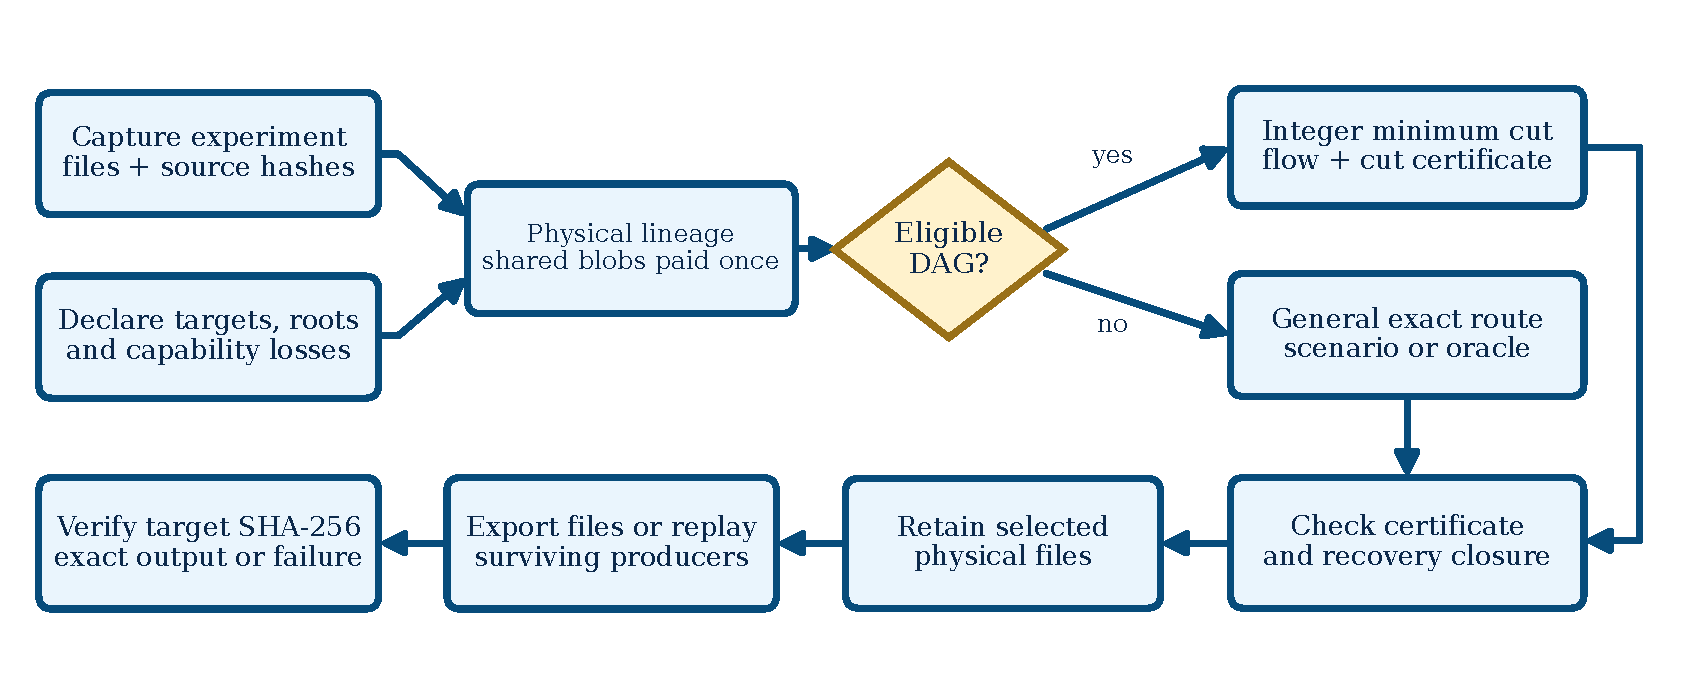
\includegraphics[width=\textwidth]{figures/methodology_rebuilt.pdf}
  \caption{RecoverML capture, file selection and recovery.}
  \Description{Captured experiments and a failure contract define physical lineage, then an eligibility check selects minimum cut or general exact optimization. The system checks the certificate, retains selected files and later replays or exports targets before checking their hashes.}
  \label{fig:method}
\end{figure*}

\subsection{Captured history and physical file identities}

Each logical node records an operation with its inputs, parameters, output hash and size, along with whether it can run again. The environment record keeps package versions and implementation hashes for supported operators and arrays and supported models use recorded serialization so exact recovery requires the same bytes rather than similar model accuracy.

Several logical nodes can refer to one physical file, so the planner pays for it only once. Let $B$ contain the captured physical blobs and let $w_b$ be the nonnegative size of blob $b$ with $\beta(p)$ giving the physical output of producer $p$ and $D(p)$ listing its physical inputs. Several producers may supply one blob, but each needs all its inputs while a node that cannot run again stays in the history without adding a recovery path.

Mandatory roots $R\subseteq B$ must remain stored and the protected targets are $T\subseteq B$, which can include models, probability arrays or older features needed for investigation. Every method receives the same manifest and roots, and recovery uses only selected files and surviving producers to reconstruct the original targets.

\subsection{Recovery contract and byte objective}

The capability map puts replayable producers into loss groups and producers that use the same entry point may share a group while ungrouped producers remain available. For the group set $G$ and loss bound $k$, the allowed losses are
\begin{equation}
  \mathcal{F}_k=\{F\subseteq G: |F|\leq k\}.
  \label{eq:faults}
\end{equation}
The requirement covers processing loss while stored files and mandatory roots remain intact and a changed environment or corrupt file causes a refusal when safe recovery cannot be proved.

For a retained set $S$, recovery begins with $A_0=S$ and adds the output of each surviving producer once all its inputs are available:
\begin{equation}
 A_{i+1}=A_i\cup\{\beta(p):p\text{ survives }F,\ D(p)\subseteq A_i\}.
 \label{eq:closure}
\end{equation}
Recovery stops at the least fixed point $\operatorname{cl}(S,F)$ and starting from stored files prevents an unsupported cycle from counting as a recovery path. The complete file selection problem is
\begin{align}
  \min_{S\subseteq B}\quad & m+\sum_{b\in S}w_b \label{eq:objective}\\
  \text{subject to}\quad & R\subseteq S,\nonumber\\
  &T\subseteq\operatorname{cl}(S,F)\quad\forall F\in\mathcal{F}_k,\nonumber
\end{align}
Here $m$ is the size of the fixed manifest and serialized contract and reported storage counts roots and metadata once.

\subsection{General exact formulations}

The scenario formulation uses one set of binary file selection variables for all allowed losses and records which files and producers remain available in each case. Rank constraints require a producer's inputs to be available first, preventing an unsupported cycle from appearing to recover itself. The solver minimizes the file cost in Equation~\ref{eq:objective} and a grounded recovery check tests the chosen store.

The second formulation starts with a storage master that has one selection variable $x_b$ for each physical blob. An oracle searches for an allowed loss $F$ and a closed set $C$ that contains the stored files but misses a target, where closed means every surviving producer with inputs in $C$ also has its output there. This witness shows that the store fails under $F$, so every valid store must satisfy
\begin{equation}
  \sum_{b\in B\setminus C}x_b\geq 1.
  \label{eq:cut}
\end{equation}
The master adds this constraint and searches again for a cheapest store. Once it proves a minimum and the oracle finds no failing loss, the selected store is feasible and optimal within the recorded model while timeouts and invalid solutions remain unknown. The master and oracle design follows established hitting set and abduction methods~\cite{hittingset}.

RecoverML checks binary values, the objective, roots and learned constraints before accepting a solver result. It first tries the DAG route below and otherwise uses the scenario formulation for at most 64 allowed scenarios, moving to the master and oracle route above that number.

\subsection{Guarded DAG specialization and its certificate}

The faster route requires a physical dependency DAG after mandatory roots are treated as available with at most one replayable producer for every optional blob. The guard rejects cycles and multiple producers of one physical output even when two logical producers wrote identical bytes.

For this subclass, universal recovery when $k\geq1$ is equivalent to recovery with all grouped producers disabled together:
\begin{equation}
 \bigcap_{F\in\mathcal{F}_k}\operatorname{cl}(S,F)
   =\operatorname{cl}(S,G).
 \label{eq:collapse}
\end{equation}
The equality describes a fixed store without adding simultaneous loss of all groups to the runtime contract. In topological order, a stored blob is available and an unstored blob whose producer may fail is not available under every allowed loss while an ungrouped producer can supply its output whenever all its inputs are available. Disabling all grouped producers gives the same universal rule and when $k=0$ no producer is disabled.

After the reduction, an unstored blob without a surviving producer becomes a failure source. Failure can pass through dependencies until a stored blob stops it, so protecting targets becomes a weighted vertex cut between failure sources and targets. Each optional blob becomes an input vertex and an output vertex joined by an edge of capacity $w_b$ while dependency and terminal edges receive capacity
\begin{equation}
  M=1+\sum_{b\in B\setminus R}w_b.
\end{equation}
Keeping every optional blob costs less than cutting an $M$ edge, as required by the standard vertex splitting construction~\cite{flow}. Roots and fixed metadata are then added to the selected file cost.

NetworkX finds an integer maximum flow and a cut and the checker verifies edge capacities and flow conservation before removing the chosen stored vertices and checking that no failure source can reach a target. The total weight of the stored optional blobs must equal the feasible flow value because the cut gives an upper bound and the flow gives a matching lower bound. A separate grounded recovery check then confirms that the store protects the targets.

The reduction does not cover every AND/OR history. Two producers in different groups may each recover a target after one group is lost, even though disabling both would prevent recovery and an unsupported physical cycle also breaks the cut argument. The guard sends these histories to a general exact route.

\subsection{Components and recovery execution}

An optional decomposition removes mandatory roots from the live dependency graph and solves the components containing targets separately, then combines their selected files and pays for global roots and metadata once. Solver projections are not saved as capture manifests and shared loss labels remain safe because each component is checked against every allowed loss relevant to it. For one optional target whose producers depend only on roots, a direct rule allows it to be omitted when an ungrouped producer exists or the number of distinct producer groups exceeds $k$.

For a recovery request, the executor finds a grounded path from stored files through surviving producers and follows dependency order. Each request has its own memo and trace and every loaded or recovered file must match its recorded hash with explicit errors for missing or corrupt files and source mismatches. The general restorer checks its supported runtime before loading values and never uses a producer declared unavailable.

When all requested targets are stored, direct export checks their sizes and SHA-256 identities and writes the outputs without loading a model. A missing target sends the request to ordinary replay while a corrupt stored target causes an error.

\subsection{Publication and concurrent recovery}

The durable publisher writes selected blobs, the manifest and the contract to a sibling directory, flushes files and POSIX directories, then atomically renames that directory to the final path on the same filesystem. One publisher owns each destination and readers use only the final path, so stopping the process before rename exposes no store and stopping it after rename leaves a complete store. Published files are read only and each request owns its restorer, memo, trace and output directory with success requiring exact target hashes.

\section{Experimental Setup}
\label{sec:experiments}

The experiments examine which files remain necessary under different loss requirements and whether other methods choose the same stores, then measure planning and actual recovery separately. Table~\ref{tab:workloads} lists the fixed studies, where one captured history may appear under several contracts or policies and the artifact saves their protocols and source snapshots~\cite{artifact}.

\begin{table*}[t]
\caption{Workloads and comparison design.}
\label{tab:workloads}
\centering\small
\begin{tabular}{p{.18\textwidth}p{.23\textwidth}p{.13\textwidth}p{.37\textwidth}}
\toprule
Study & Data and model family & Captures; versions & Main comparison or control\\
\midrule
Shared loss study & Wine and Breast Cancer; logistic regression & 36; 4/16/64 & Three seeds, two capture boundaries, two failure groupings, nine policies\\
Native recovery & Fresh captures of the same recipe grid & 36; 4/16/64 & RecoverML versus native batched DVC at identical paid payloads; three paired repetitions\\
Published rules & Public tabular data; original HYPPO components and HELIX rule adapter & 28; varied & Two loss bounds give 56 cases; 3,344 requests per policy at the common robust byte limit\\
Encoded storage & Six public datasets plus scientific, cloud and retinal transfers & 446 conditions & Previous flat and delta choices, flat joint archive and local search with the same formats; two Letter cases unmeasured\\
Recovery census & Six public datasets and four deterministic recipes & 72 captures & Three loss contracts, two request sizes and two interfaces; 864 paired configurations at equal paid payloads\\
Scientific matrix & Iris, Digits and Diabetes; four recipes & 8; 3 each & Two seeds, two loss scopes, three bounds, five budgets, eight policies\\
Retinal histories & 20 STARE images; logistic regression and forest & 18; 2/8/16 & Two target modes, three availability contracts, five retention policies\\
Large payload & UCI Letter; trained random forests & 1; 16 & Preprocessing versus broad loss and canonical versus compressed representation\\
Final runtime scaling & Breast Cancer linear and Digits PCA and neighbor histories & 6; 1/4/16 & Root replay or retained target export; 1/2/4/8 threads or 1/2/4 process replicas; three repeats\\
\bottomrule
\end{tabular}
\end{table*}

\subsection{Histories and declared processing changes}

The shared loss grid uses Wine and Breast Cancer from scikit-learn~\cite{datasets} with a stratified split assigning 75\% to training and 25\% to testing under seeds 20261016, 20261017 and 20261018. Two disjoint feature views are standardized using training data only and logistic regression versions cover regularization from $10^{-3}$ to $10^3$. One capture boundary lets later steps consume both views directly and the other also stores their concatenated matrix.

We test each history with separate preprocessing groups and then one group covering both standardization steps, keeping $k=1$ and the captured bytes the same. The shared loss study followed a favorable pilot, so its complete grid keeps small histories and explicit concatenation controls.

The scientific matrix adapts Iris feature union, Digits PCA, Diabetes polynomial features and Digits forests with two seeds and three versions giving eight captures. We test them under preprocessing and broad loss with $k\in\{0,1,2\}$ and set five budgets from fixed roots and metadata plus 0, 10, 25, 50 or 100\% of optional target snapshot bytes. The budgets therefore do not depend on a later optimum and eight methods give 1,920 method and budget rows.

The retinal study uses all 20 STARE fundus images and Hoover vessel annotations~\cite{stare}. Images become $64\times64$ RGB with 15 training images, five test images and 6,000 sampled training pixels. Three seeds, two model families and three history lengths give 18 captures and an aligned extractor replaces a legacy feature shift of three pixels so the feature bytes change. We protect models and predictions and sometimes investigation features under contracts for intact processing, loss of the old extractor or loss of training and prediction. Model settings also change between versions.

The large study uses all 20,000 UCI Letter observations with 16 features and 26 classes~\cite{letter}. Seed 20261015 gives a stratified split of 15,000 training and 5,000 test observations and MinMax scaling and chi-squared selection fitted on training data keep 12 features. Sixteen trained forests combine 64/128/192/256 trees with two feature sampling settings and two model seeds, without padding or duplicated payload added to meet a storage target.

\subsection{Comparators and budget fairness}

The exact comparators solve the same complete recovery problem while robust greedy adds the largest grounded coverage gain per byte. The stronger local search also removes unnecessary files from a full store and tries exchanges of one file followed by pruning, allowing at most two exchange passes. Target snapshots keep protected outputs directly and the manual frontier control uses knowledge of each workflow to choose its smallest feasible frontier.

HYPPO rank and frequency use a pinned released component and HELIX uses a documented rule adapter with the same executor and byte accounting even though their rules were designed for reuse. In the cloud grid they receive the exact minimum total byte budget while robust heuristics and snapshots can use the full candidate allowance to compare complete stores. The scientific matrix gives every method the same fixed budget at each point, so it answers a different comparison question.

The separate matrix of 56 cases gives RecoverML, both HYPPO functions and six HELIX settings the same robust byte limit. HYPPO uses its pinned released component through a physical file adapter and HELIX uses a documented streaming rule reimplementation at 50, 200 and 800 MiB/s with both recorded tie orders. We report a HELIX control with the larger snapshot budget separately and all policies use the same grounded recovery executor so the results compare file selection decisions~\cite{artifact}.

The native DVC study uses DVC 3.67.1 with certified optimal retained payloads and excludes selection time. A single downstream batch stage avoids starting Python separately for every model and DVC can skip that stage when the correct target cache objects are retained. Before each trial both methods have the same paid physical payloads and no unpaid downstream cache objects with hard links for common retained files and byte checks based on distinct inodes. We record DVC configuration separately from the common payload objective and both authored workers can use the exact file export helper.

The encoded storage study keeps the earlier flat optimum as a candidate and adds exact prefix and suffix deltas with their bases and headers charged, along with a measured joint archive of retained canonical payloads. The final selector computes the flat exact, delta exact, flat local, delta local and separately compressed choices, then keeps the smallest complete store. We compare it with the earlier flat and delta implementation, a joint archive of the flat optimum and local search using all offered formats. The first choice among three candidates lost three conditions to the stronger local control, so we disclosed that result and added both local plans. Every row in the later table uses the final choice among five candidates and the artifact keeps the original losses~\cite{artifact}.

The later storage catalogue contains 216 primary, 48 scientific transfer, 72 cloud conditions across three seeds and 108 retinal conditions, plus two Letter conditions without complete paired storage values. Byte totals include metadata, mandatory roots and delta bases and saved file and export checks verify exact identities. The joint archive is decoded into memory and uses a temporary retained store for replay.

The broader native DVC census uses 72 captures from six datasets, four recipes and three history lengths. Three loss contracts, two request sizes and command line or warm API access give 864 configurations, each measured in three paired repetitions with randomized order and the same certified optimal retained payloads. The elapsed call includes the requested file inventory and hash checks but excludes capture, planning and setup and OS caches are not flushed. A separately coded direct executor measures the cost of DVC orchestration~\cite{artifact}.

\subsection{Machines, repetitions and recorded outcomes}

Each of three Linux GitHub runners handles one fixed seed block in the shared loss study, exposing four virtual CPUs on AMD EPYC 7763 hosts. The native study also uses runners with four CPUs with EPYC 9V74 for one block and EPYC 7763 for two. The environment uses Python 3.12.15, NumPy 2.3.5, SciPy 1.17.0 and scikit-learn 1.8.0 with one BLAS thread for numerical execution.

Each cloud planner has three timed calls per case and the earlier replanning study with 48 conditions has five. General solver calls use a 30 s limit with a requested relative MIP gap of zero and allow 120 s in Letter while the polynomial flow route has no hard interruption deadline. The native recovery comparison uses three paired trials with deterministically randomized method order and its main elapsed time includes cold subprocess and CLI startup and the final common SHA-256 check. Setup and planning are excluded, worker timings and CPU are logged separately and OS page caches are not flushed.

Each actual request records whether the expected target identities were recovered, a deficient store was correctly blocked or an unexpected outcome occurred. Methods selecting identical stores share explicitly attributed execution evidence, so adding their totals would overcount physical requests. We calculate ratios from method medians within each history before summarizing across histories.

The final file API runs on a Linux runner with four vCPUs and an AMD EPYC 9V74 processor. Breast Cancer and Digits histories have 1, 4 and 16 versions and replay from roots and export of retained targets use different measured byte totals. Each condition has three bursts of 128 requests with 1/2/4/8 threads or 1/2/4 process replicas on the same host, giving 252 trials. Each request writes to a private output directory and timings exclude warmup and planning. Throughput covers submission through completion. Service P99 measures execution and response P99 also includes queue wait with every request, source hash, machine record and independent audit saved in the artifact.

A separate ablation keeps the physical retained store and target request fixed while timing direct export, export after graph and contract setup and the same export followed by object conversion. It uses two workloads, three history lengths, three repeats and 64 paired requests per repeat, rotating arm order within each request and checking outputs and hashes before summarizing timings.

\section{Results}
\label{sec:results}

\subsection{Storage choices under shared preprocessing loss}

The two exact formulations agree on all 72 history and contract minima and 216 repeated planning calls include checked flow proofs. RecoverML uses fewer bytes than strong local search in six of 36 separate loss cases and ties in 30 with each win saving 129 serialized bytes. Under shared loss it wins nine of 36 and ties 27 with no losses, as Table~\ref{tab:cloud} records and Figure~\ref{fig:shared} shows for all shared loss cases. The median saving over the full grid is zero and the manual best frontier matches every exact minimum. W and B in the figure mean Wine and Breast Cancer and each version count has three seed points with reductions based on the full paid store size.

\begin{table}[t]
\centering\small
\caption{Storage choices against strong local search.}
\label{tab:cloud}
\begin{tabular}{lrrrr}
\toprule
Loss grouping & Wins & Ties & Losses & Max. reduction\\
\midrule
Separate & 6 & 30 & 0 & 0.1942\%\\
Shared & 9 & 27 & 0 & 48.7380\%\\
\bottomrule
\end{tabular}
\end{table}

\begin{figure*}[t]
\centering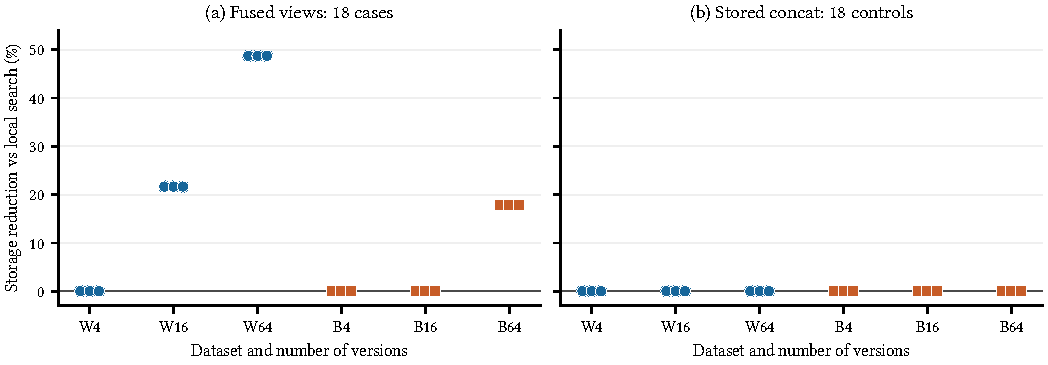
\includegraphics[width=\textwidth]{figures/shared_storage.pdf}
\caption{Storage reduction under shared preprocessing loss.}
\Description{Two panels compare storage with strong local search for fused views and stored concatenation in every Wine and Breast Cancer setting. Nine fused cases save bytes and every concatenation control ties.}
\label{fig:shared}
\end{figure*}

The nine shared loss wins occur across all three seeds in fused Wine histories with 16 or 64 versions and fused Breast Cancer histories with 64 versions. In the largest case RecoverML stores 138,618 bytes and local search stores 270,411, saving 131,793 bytes or 48.7380\%. The difference is about 132 KB in absolute size while the separate Letter study measures a larger byte saving.

Replacing many models and predictions may require both standardized views together, so an exchange of one file can miss the useful joint choice. Recording their concatenation gives local search that choice as a single file and closes the gap in all 18 concatenation controls while the manual frontier also reaches every minimum.

\subsection{Coverage and the meaning of a complete contract}

At the cloud grid's exact minimum budget, RecoverML completes recovery in 36/36 histories per loss grouping, HYPPO rank in 18/36, HYPPO frequency in 21/36 and the HELIX rule in 15/36. The robust full store controls stay feasible but may retain more bytes. The physically unique cloud requests give 16,110 exact results and 3,542 expected blocks out of 19,652 with zero unexpected outcomes and all requests attributed to RecoverML are exact while deficient adapter stores account for the blocks.

\subsection{Published decision rules at one robust storage limit}

Every policy in the matrix of 56 cases receives the same robust byte limit and 3,344 historical requests and RecoverML restores all 3,344. Table~\ref{tab:published} reports both HYPPO components and every tested HELIX speed and tie order with HYPPO restoring 2,240 and 2,291 requests and the best HELIX setting at the common limit restoring 1,940. A separate HELIX control restores 2,437 of 3,344 with the larger target snapshot budget and stays outside the common limit comparison~\cite{artifact}. The HYPPO rows use released ranking components through an adapter and HELIX uses the reimplemented rule with the same executor for all.

\begin{table}[t]
\caption{Exact recovery with the same robust byte limit.}
\label{tab:published}
\centering\small
\begin{tabular}{lrr}
\toprule
Policy & Exact & Requested\\
\midrule
RecoverML & 3,344 & 3,344\\
HYPPO rank & 2,240 & 3,344\\
HYPPO frequency & 2,291 & 3,344\\
HELIX 50 MiB/s, capture order & 1,940 & 3,344\\
HELIX 50 MiB/s, reverse order & 1,940 & 3,344\\
HELIX 200 MiB/s, capture order & 1,681 & 3,344\\
HELIX 200 MiB/s, reverse order & 1,681 & 3,344\\
HELIX 800 MiB/s, capture order & 1,673 & 3,344\\
HELIX 800 MiB/s, reverse order & 1,673 & 3,344\\
\bottomrule
\end{tabular}
\end{table}

Across the 28 related histories, every tested method restores all 320 requests without an outage in the lossless subset. With one disabled group RecoverML restores 960/960 requests, HYPPO rank and frequency restore 729/960 and 818/960 and the HELIX 50 MiB/s capture setting restores 722/960. With two disabled groups the respective counts are 480/480, 278/480, 350/480 and 271/480. The difference appears under the declared losses, although cases with rounded imports may also reflect the difference between protecting old targets and choosing files for future reuse.

The scientific matrix gives each method 240 conditions and 4,560 requests and Table~\ref{tab:scientific} distinguishes complete recovery of a condition from the number of individual requests recovered. RecoverML and local search each complete 128 conditions, although local search returns more individual targets across the budgets. RecoverML optimizes complete recovery when feasible and local search matches all 48 exact storage minima at full budget.

\begin{table}[t]
\centering\small
\caption{Recovery in the scientific fixed budget matrix.}
\label{tab:scientific}
\begin{tabular}{lrr}
\toprule
Method & Complete conditions & Exact requests\\
\midrule
RecoverML exact & 128 & 1,734\\
Scenario exact & 128 & 1,734\\
Robust greedy & 112 & 2,221\\
Robust local & 128 & 2,324\\
HYPPO rank & 104 & 1,989\\
HYPPO frequency & 100 & 1,856\\
HELIX rule & 96 & 1,700\\
Target snapshots & 112 & 1,862\\
\bottomrule
\end{tabular}
\end{table}

\subsection{Planning cost and component checks}

In the new cloud grid, the median paired ratio of local planning time to RecoverML time is 11.92 under separate loss and 16.88 under shared loss and the corresponding scenario ratios are 2.28 and 1.73. These measure planning wall time separately from artifact recovery. The older timing study with 48 conditions keeps the original minima and gives a 4.20 median ratio against local search with RecoverML faster in 44 conditions and slower in four.

Figure~\ref{fig:planning} gives one point per condition and a black median bar from five planning repetitions per method. RecoverML is faster than local search in all 36 eligible DAG cases with a median ratio of 6.27 while the 12 fallback cases give medians of 1.64 against local search and 0.93 against scenario exact. A ratio above one favors RecoverML, so the fallback is slower than scenario exact at its median and four comparisons with local search are also slower.

\begin{figure*}[t]
\centering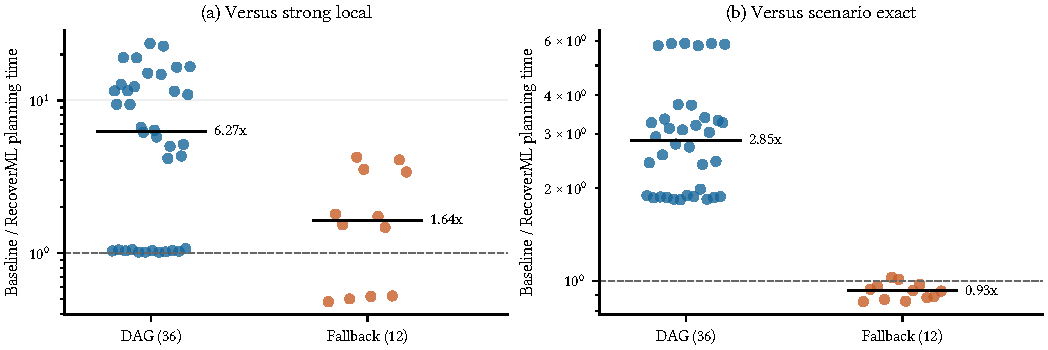
\includegraphics[width=\textwidth]{figures/planner_timing.pdf}
\caption{Planning time ratios across 48 conditions.}
\Description{Two scatter panels show local and scenario planning time ratios across 36 eligible DAG conditions and 12 fallback conditions, using a reference line at one.}
\label{fig:planning}
\end{figure*}

A separate finite guard validation enumerates 2,275 DAG specifications with four artifacts, comparing 18,200 closures for fixed stores and 127,400 minimum cut optima against exhaustive search without disagreement.

The component study records 154 rows, including 110 under the same contract and all 99 certified objective comparisons under that contract agree. All 1,452 enumerated fault certificate checks and six indexed versus reference chain comparisons also agree, although decomposition is slower than the route without decomposition in six of eight settings from public recipes. A separate annotation study covers 5,760 conditions and changes selected sets in 298/4,608 cost profile comparisons and 312/2,880 access weight comparisons, showing that adapter outcomes depend on the stated annotations.

\subsection{Native recovery at identical retained storage}

The final native comparison completes 216 subprocess commands for full histories and 12,096 exact target hash checks with lower median elapsed time for RecoverML in all 36 histories. Figure~\ref{fig:native} places the median of three trials for each history against an equality line and shows paired ratios separately for histories needing replay and those with stored targets. Timing includes startup and verification but excludes setup and planning and OS caches are not flushed.

For the 18 histories needing downstream computation, the median paired ratio of DVC time to RecoverML time is 2.1856 and ranges from 1.7215 to 2.5109. For the 18 histories with retained targets, it is 9.9067 and ranges from 8.9527 to 11.3402. The medians of absolute times across histories are 1.663 s for RecoverML and 4.146 s for DVC with recomputation and 0.0633 s versus 0.6056 s with retained targets.

\begin{figure*}[t]
\centering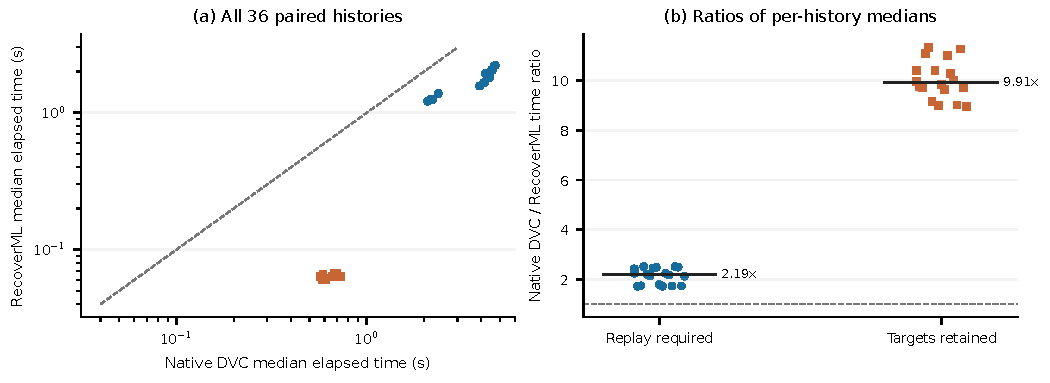
\includegraphics[width=\textwidth]{figures/native_recovery.pdf}
\caption{Native DVC and RecoverML recovery times.}
\Description{A scatter plot with logarithmic axes compares DVC and RecoverML elapsed time for every history and places every point below equality. The second panel shows paired time ratios for targets that need replay and targets that are already retained.}
\label{fig:native}
\end{figure*}

Direct export avoids numerical startup when replay is unnecessary and both workers can use the same helper. DVC still pays for its native command and stage handling, so the large ratio for retained targets describes these cold command integrations. An earlier revision with corrected paid cache accounting gave mixed results with RecoverML winning all 18 recomputation cases and DVC winning all 18 retained target cases. We added the export improvement after that result and tested it on a fresh full grid.

\subsection{Complete encoded storage comparison}

Table~\ref{tab:encoded} compares the final choice among five candidates with four storage controls using total paid bytes. There are 446 conditions, but one Letter case has only the selected store and another lacks its original archive, leaving 444 measured pairs. Smaller, equal and larger count each comparison and the 10\% column uses all 446 conditions. Because the final choice includes the old plan and both local plans, it cannot use more bytes than those candidates. The earlier choice among three candidates had 20 wins, 421 ties and three losses against the stronger local control using the same formats and adding both local candidates corrected those losses~\cite{artifact}.

\begin{table*}[t]
\caption{Storage outcomes for the choice among five candidates.}
\label{tab:encoded}
\centering\small
\begin{tabular}{lrrrrrr}
\toprule
Comparator & Smaller & Equal & Larger & Unmeasured & Median saving & 10\%+\\
\midrule
Previous flat optimum & 244 & 200 & 0 & 2 & 0.094\% & 52\\
Previous flat or delta choice & 214 & 230 & 0 & 2 & 0\% & 47\\
Joint archive of flat optimum & 233 & 211 & 0 & 2 & 0.056\% & 5\\
Local search with all offered formats & 20 & 424 & 0 & 2 & 0\% & 9\\
\bottomrule
\end{tabular}
\end{table*}

The largest reduction against the previous flat optimum is 89.84\%, from 1,457,715 to 148,050 bytes in \path{digits/pca_neighbors/v16/broad}. Against the local control using the same formats, the largest gap is 70.17\%, from 118,126 to 35,242 bytes in \path{shared/wine-s20261016-v64-concat0}. Most of that local gap existed before joint compression, so it does not show a new 70\% compression gain. The median saving against local search is zero and only nine of 446 conditions reach 10\% savings. The inherited broad improvement test requires at least 10\% saving in 90\% of histories per stratum and passes in zero of 72 strata.

The exact reference using the same formats ties the measured flat and delta optima within their declared candidate inventories, and the manual best frontier ties all 36 minima in the earlier shared loss study. Joint compression adds further storage choices, and the corrected selector reduces bytes in the reported conditions while matching the retained candidates in the remaining measured comparisons.

The independent release audit rebuilds archive controls from saved canonical payloads and reproduces both local selectors. It reconciles 8,592 saved file and export checks, comprising 5,061 selected file checks and 3,531 retained target export checks including repeated artifacts. All 29 cloud jobs and the final audit passed~\cite{artifact}.

\subsection{Broader native DVC recovery census}

In the later census, the tested native DVC integration takes more than 1.10 times the RecoverML elapsed time in all 864 configurations, meeting the prespecified threshold. The median paired ratios of DVC time to RecoverML time are 1.6952 for the 432 command line configurations and 48.3212 for the 432 warm API configurations. All 7,776 trials restore the requested files exactly and the ledger checks 54,540 requested file hashes~\cite{artifact}.

The direct executor control helps explain the DVC difference with a median elapsed time divided by RecoverML time of 0.9929 that slightly favors the direct control. RecoverML reaches an improvement of 1.10 times in only 21 of 864 direct comparisons and is at least 1.10 times slower in 48, so the native DVC difference mainly measures orchestration in these integrations.

\subsection{Historical processing change and large payloads}

The retinal study completes 10,920 exact requests across 540 method rows with no unexpected errors and Figure~\ref{fig:retinal} includes all 108 storage conditions. Colors identify the availability contract, circles and triangles identify logistic regression and forests and small offsets separate the three seeds. Adding investigation features changes the protected file set while broad training and prediction loss can require target snapshots. Exact retention saves bytes against target snapshots in 90 cases and ties in 18, improves on simple greedy in 12 and ties in 96 and matches strong local search and a simple frontier rule in all 108 cases. The conditions share the same 20 public images.

\begin{figure*}[t]
\centering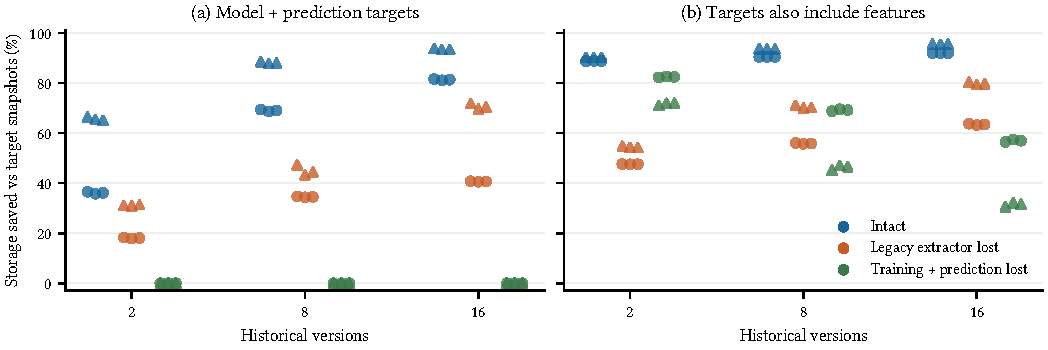
\includegraphics[width=\textwidth]{figures/retinal_storage.pdf}
\caption{Retinal storage savings across 108 conditions.}
\Description{Two panels show storage savings against target snapshots for three history lengths with intact processing, loss of the legacy extractor, or loss of training and prediction.}
\label{fig:retinal}
\end{figure*}

The largest retinal saving against snapshots is 12,316,663 bytes in an intact forest history that protects investigation features. A separate native control removes the legacy module before reproduction and confirms it is still absent afterward while recovering all 32 protected targets exactly. A manually retained DVC frontier matches the common objective of 2,523,881 bytes.

Under preprocessing loss, the Letter canonical store falls from 3,669,545,821 to 4,829,269 bytes, saving 3,664,716,552 bytes or 99.8684\%, which is more than 3.66 GB. With gzip it falls from 291,175,536 to 568,375 bytes and saves 290,607,161. Figure~\ref{fig:letter} plots decimal MB on a logarithmic axis with each RecoverML bar beside its target snapshot control. Strong robust heuristics match the preprocessing optimum and broad loss gives no canonical or gzip saving while native pickle and native gzip controls have different byte identities and are recorded separately.

\begin{figure*}[t]
\centering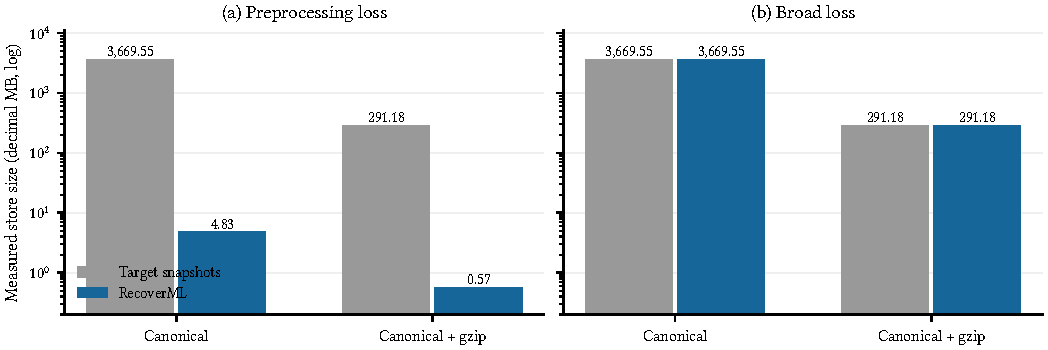
\includegraphics[width=\textwidth]{figures/letter_storage.pdf}
\caption{Letter store sizes under preprocessing and broad loss.}
\Description{Paired bars compare canonical and gzip store sizes under preprocessing and broad loss, showing smaller stores under preprocessing loss and equal stores under broad loss.}
\label{fig:letter}
\end{figure*}

The Letter replay ledger contains 48 exact requests across three unique stores with all preprocessing groups disabled, which is a stronger stress than the $k=1$ selection contract. Broad loss is checked structurally. In the descriptive preprocessing replay, mean frontier recovery takes 6.65 s per version and snapshot loading takes 2.12 s. All 16 trained forests are included and their accuracy on held out data ranges from 95.0\% to 95.64\%.

\subsection{Concurrency, tail latency and process crashes}

The final file API recovers all 32,256 requests exactly across 252 audited trials and Figure~\ref{fig:performance} compares each dataset, version count and mode with its result with one worker. Points give the medians of six ratios for fixed cases and shading shows their range. Storage differs between modes: at 16 versions, stores containing only roots and stores containing target files cost 172,570 and 205,679 bytes for Breast Cancer and 975,357 and 3,117,275 bytes for Digits.

\begin{figure*}[t]
\centering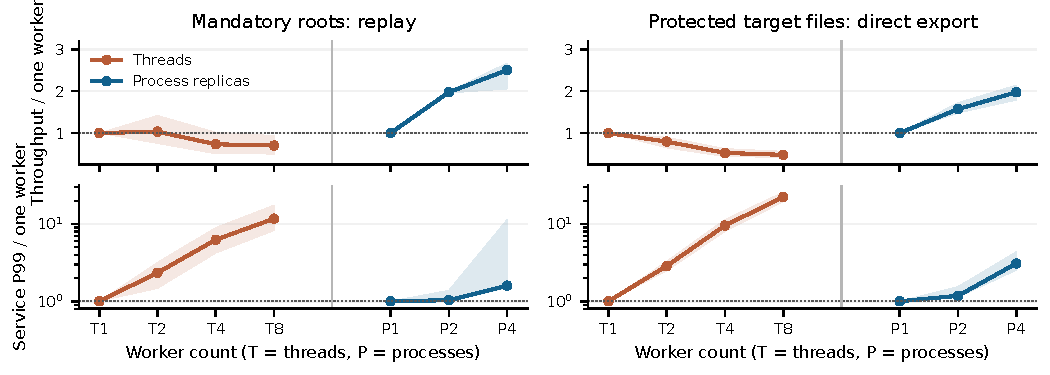
\includegraphics[width=\textwidth]{figures/runtime_scaling.pdf}
\caption{Final file API throughput and service P99 relative to one worker.}
\Description{Four vector panels show the median and range of throughput and service P99 ratios across fixed cases with small dots for all 18 trial P99 ratios at each worker count. Four process replicas on the same host raise throughput in both retention modes and eight threads lower it while tail latency grows with concurrency.}
\label{fig:performance}
\end{figure*}

Four process replicas raise throughput in all six fixed cases per mode, giving median ratios of 2.50 for replay and 1.97 for export. Eight threads lower throughput in all 12 cases with median ratios of 0.70 and 0.48 while the median service P99 ratios at four processes are 1.59 and 3.09 and those at eight threads are 11.75 and 22.38. Figure~\ref{fig:performance} includes all 18 trial P99 ratios at each worker count and the saved requests give individual service times and queue waits. The earlier prototype has a separate record of 5,400 exact requests across 54 trials.

We also run replay from roots on independent Linux runners with one, two or four replicas each capturing the same declared Digits history of 16 versions. Over three synchronized rounds per configuration, all 2,688 requests match their own runner's recorded target hashes. Median aggregate throughput is 36.4, 71.4 and 144.7 requests/s, giving 1.96 and 3.97 times the rate of one runner and the rate across four runners reaches 82\% of the sum of its individual rates. The runners have two CPU variants and produce two target hash sets, so the ratios describe provisioned capacity on different hardware rather than speedup on identical hardware. Each replica uses its own immutable store.

The ablation of RecoverML paths using the same store recovers all 3,456 requests exactly. Across 18 matched workload, length and repeat groups, graph and contract setup makes median request time 3.28 times direct export and adding object conversion with its source reread makes it another 1.32 times the setup and export path. Both costs appear in all 18 group medians, showing why direct export of retained files is the measured fast path within RecoverML.

The process crash tests kill a child just before or after publication, leaving the final path absent before rename and fully verifiable after it. A separate test has 32 readers recover exact bytes from one immutable store into private outputs and the artifact maps the publication states and reader rules on one filesystem to these tests~\cite{artifact}.

\section{Discussion and Reproducibility}
\label{sec:discussion}

RecoverML first protects complete recovery and then minimizes stored bytes with recovery time measured separately. The manual frontier ties and faster snapshot loads show how this objective affects the preferred choice. The repository keeps source hashes, captured file identities, raw timings, solver records and analysis scripts~\cite{artifact} and its paper build checks the six measured figures against saved calls, trials, manifests and file ledgers before regenerating all seven vector figures. Fresh runs use new output directories and none of the studies required a GPU.

\section{Limitations}

The evaluation uses public datasets and histories built for this project, so its win rates do not estimate production performance. Seeds and requests reuse captures, retinal histories are not strict nested prefixes, and requests for the latest version and all versions coincide for histories with one version. The shared loss grid followed a favorable pilot and the choice among five storage candidates was corrected after the stronger local control exposed three losses.

The recovery guarantee assumes complete recorded dependencies, intact stored files and a supported replay environment. Certificates apply to the stated file model and the exhaustive guard checks cover finite graphs, while general exact optimization grows with the allowed loss scenarios. Six original scientific captures without forests lack a completed global source guard after an interruption, although their snapshots, request guards and raw reconciliation remain available. One original Letter archive container is missing, while all four frontier payloads have matching hashes in a documented replacement.

HELIX and HYPPO comparisons cover adapted selection components and native DVC timings cover authored integrations. Exact certificates cover the declared flat and delta inventories rather than every possible jointly compressed retained set. Compression time, random access cost, peak memory, annotation effort, deployment cost and capability loss frequency remain unmeasured. Crash tests cover processes and publication on one filesystem, while larger neural states, software migration, networked shared storage, recovery from power loss and distributed crash consistency need further study.

\FloatBarrier
\section{Conclusion}

RecoverML records old ML files and chooses a checked store that keeps protected outputs recoverable after specified processing losses. At the same robust byte limit it restores all 3,344 requests per policy in the study of decision rules across 56 cases, where the tested HYPPO components and HELIX rule settings recover fewer. The choice among five storage candidates reduces bytes against the earlier flat optimum in 244 of 444 measurable cases and against local search using the same formats in 20 with 424 local ties. The native DVC census also favors RecoverML with the same stored files while a direct executor is close in time and manual or exact choices using the same formats match the relevant storage minima.

\balance
\bibliographystyle{ACM-Reference-Format}
\bibliography{references}

\end{document}
